\documentclass[11pt,a4paper]{article}
\usepackage[margin=2.2cm]{geometry}
\usepackage{lmodern}
\usepackage[T1]{fontenc}
\usepackage[utf8]{inputenc}
\usepackage{amsmath,amssymb,amsthm}
\usepackage{booktabs,array,tabularx,longtable}
\usepackage{enumitem}
\usepackage{xcolor}
\usepackage[most]{tcolorbox}
\usepackage{titlesec}
\usepackage{graphicx}
\usepackage{float}
\usepackage{adjustbox}
\usepackage{listings}
\usepackage{tikz}
\usetikzlibrary{arrows.meta,positioning,calc,fit}
\usepackage[font=small,labelfont={bf,color=headblue},skip=4pt]{caption}
\usepackage[colorlinks=true,linkcolor=headblue,urlcolor=blue!50!black]{hyperref}

\definecolor{headblue}{RGB}{38,70,120}
\definecolor{codebg}{RGB}{248,248,246}
\titleformat{\section}{\Large\bfseries\color{headblue}}{\thesection}{0.8em}{}[{\color{black}\titlerule}]
\titleformat{\subsection}{\large\bfseries\color{headblue}}{\thesubsection}{0.8em}{}
\titleformat{\subsubsection}{\normalsize\bfseries\color{headblue}}{\thesubsubsection}{0.8em}{}
\titlespacing*{\section}{0pt}{12pt}{6pt}
\titlespacing*{\subsection}{0pt}{9pt}{3pt}
\setlength{\parindent}{0pt}
\setlength{\parskip}{5pt}
\setlist{itemsep=1pt,topsep=2pt}
\renewcommand{\arraystretch}{1.12}
\setlength{\emergencystretch}{3em}

\newtcolorbox{keybox}{colback=blue!3,colframe=headblue!60,boxrule=0.5pt,arc=2mm,left=2mm,right=2mm,top=1mm,bottom=1mm}
\newtcolorbox{insum}{colback=green!3,colframe=green!40!black,boxrule=0.4pt,arc=1.5mm,left=2mm,right=2mm,top=0.5mm,bottom=0.5mm,fontupper=\small}
\newcommand{\inshort}[1]{\begin{insum}\textbf{In short.} #1\end{insum}}
\newtcolorbox{example}{colback=orange!3,colframe=orange!60!black,boxrule=0.4pt,arc=1.5mm,left=2mm,right=2mm,top=0.5mm,bottom=0.5mm,fontupper=\small}
\newcommand{\code}[1]{\texttt{#1}}
\let\origunderscore\_
\renewcommand{\_}{\origunderscore\allowbreak}
\newcommand{\Fcs}{\mathrm{F}}
\newcommand{\Mcs}{\mathrm{M}}

\theoremstyle{plain}
\newtheorem{proposition}{Proposition}

\lstset{language=Python, basicstyle=\ttfamily\scriptsize, numbers=left, numberstyle=\tiny\color{gray},
  numbersep=6pt, frame=single, rulecolor=\color{black!25}, backgroundcolor=\color{codebg},
  breaklines=true, breakatwhitespace=false, columns=fullflexible, keepspaces=true, showstringspaces=false,
  keywordstyle=\color{headblue}\bfseries, commentstyle=\color{black!55}\itshape,
  stringstyle=\color{orange!60!black}, xleftmargin=14pt, framexleftmargin=2pt, aboveskip=6pt, belowskip=4pt}
\newcommand{\src}[3]{\lstinputlisting[firstline=#2,lastline=#3,caption={\texttt{\detokenize{#1}}, lines #2--#3}]{#1}}
\renewcommand{\lstlistingname}{Code}

\hypersetup{pdftitle={How the RL code works (formulation 4)}, pdfauthor={Yakshith Maddineni}}

\begin{document}

\begin{titlepage}
\centering
\vspace*{2cm}
{\LARGE\bfseries\color{headblue} How the Reinforcement-Learning Code Works\par}
\vspace{6pt}
{\Large Environment, actions, reward, network, training and solving,\\ explained line by line and compared with the MILP\par}
\vspace{14pt}
{\large Formulation 4 (personal and commercial EVs, income index)\par}
\vspace{4pt}
{\large CP 320 Operations Research for Mobility Management, course project\par}
\vspace{22pt}
{\large Yakshith Maddineni (SR 26080)\par}
{\normalsize M.Tech Smart Mobility \& Logistics Systems, IISc\par}
\vspace{6pt}
{\normalsize 26 November 2026\par}
\vfill
\begin{keybox}
\textbf{What this report is.} A reading guide to the reinforcement-learning (RL) code of formulation 4, in \code{2026-11-22\_formulation\_4/baseline\_RL/code/} (the code behind the RL results of the server job). It explains every file and every important function: what goes in, what comes out, the mathematics behind it, and the exact Python lines that do it. The environment (state, action, masks, transition), the reward function and its exact link with the MILP objective, and every constraint of the MILP and how the RL handles it are explained in detail. The report ends with one complete episode of the trained policy on a real instance, every step with real numbers, checked against the independent plan checker and against the MILP's optimal plan.

\textbf{How it relates to the other RL folders.} RL1 (formulation 3) and RL2 use the same code structure; Section~\ref{sec:versions} lists the differences. The design choices and the papers behind the method are explained in \code{RL2\_reinforcement\_learning\_method\_2/reports/RL\_implementation\_report.pdf}; the results of the formulation-4 runs are in \code{report/comprehensive\_report\_f4.pdf}.
\end{keybox}
\end{titlepage}

\tableofcontents
\newpage

%=====================================================================
\section{The big picture}

\subsection{What the RL does, in four sentences}

The MILP looks at all decisions at once and lets Gurobi search for the best combination. The RL instead \textbf{builds a plan one decision at a time}: at every step it picks one car that is not yet placed and one charger for it (a gun of a station, or a van), and the car is added at the end of that charger's queue or route. A \textbf{simulator} (the \emph{environment}) works out the start time, checks every rule, and computes exactly how much the total cost $Z$ grows because of this decision. A \textbf{neural network} (the \emph{policy}) gives a probability to every allowed decision; it learns, from many random practice instances, to give high probability to decisions that lead to cheap complete plans.

\subsection{The files}

\begin{table}[H]
\centering\small
\caption{The code of the formulation-4 RL. Paths are relative to \code{2026-11-22\_formulation\_4/}.}
\begin{tabularx}{\textwidth}{@{}>{\raggedright\arraybackslash}p{5.2cm}r>{\raggedright\arraybackslash}X@{}}
\toprule
file & lines & what it does \\
\midrule
\code{data/solomon\_data.csv}, \code{solomon\_config.csv} & -- & the dataset: positions, energies, requests, ranges, segment, $\theta$; one config row per file \\
\code{common/f4\_params.json}, \code{f4\_params.py} & 177 & customer parameters; per-car $\mu_i$, $c^a_i$, $W_i$ from segment and $\theta$ (Section~\ref{sec:data}) \\
\code{common/f4\_data.py} & 178 & reads the dataset; builds the \emph{instance dictionary} \code{J} (distances, times, coefficients) \\
\code{baseline\_RL/code/rl\_f4\_env.py} & 439 & \textbf{the environment}: tensors of a batch of instances, state, allowed actions, transition, cost increase, network inputs, greedy rule, conversion to a plan (Sections~\ref{sec:env}--\ref{sec:compare}) \\
\code{baseline\_RL/code/rl\_f4\_model.py} & 164 & \textbf{the policy network} and the \code{rollout} loop that plays episodes (Section~\ref{sec:network}) \\
\code{baseline\_RL/code/rl\_f4\_generator.py} & 145 & random practice instances made with the dataset's rules (Section~\ref{sec:generator}) \\
\code{baseline\_RL/code/train\_rl\_f4.py} & 420 & training: imitation warm-up, REINFORCE, validation, stopping, saving (Section~\ref{sec:training}) \\
\code{baseline\_RL/code/solve\_rl\_f4.py} & 302 & solving the 560 test instances with the trained model (Section~\ref{sec:solve}) \\
\code{baseline\_RL/code/test\_rl\_f4.py} & 208 & self-checks \\
\code{baseline\_RL/code/rl\_f4\_params.json} & 71 & all RL settings (network size, learning rates, batch sizes, stopping) \\
\code{common/check\_plan\_f4.py} & 142 & independent checker: every rule of the MILP and $Z$ recomputed from scratch \\
\code{common/results\_io\_f4.py} & 523 & scores a plan with the checker and writes \code{runs.csv} / \code{plan.csv} (same for MILP and RL) \\
\bottomrule
\end{tabularx}
\end{table}

\subsection{How the pieces work together}

\begin{figure}[H]
\centering
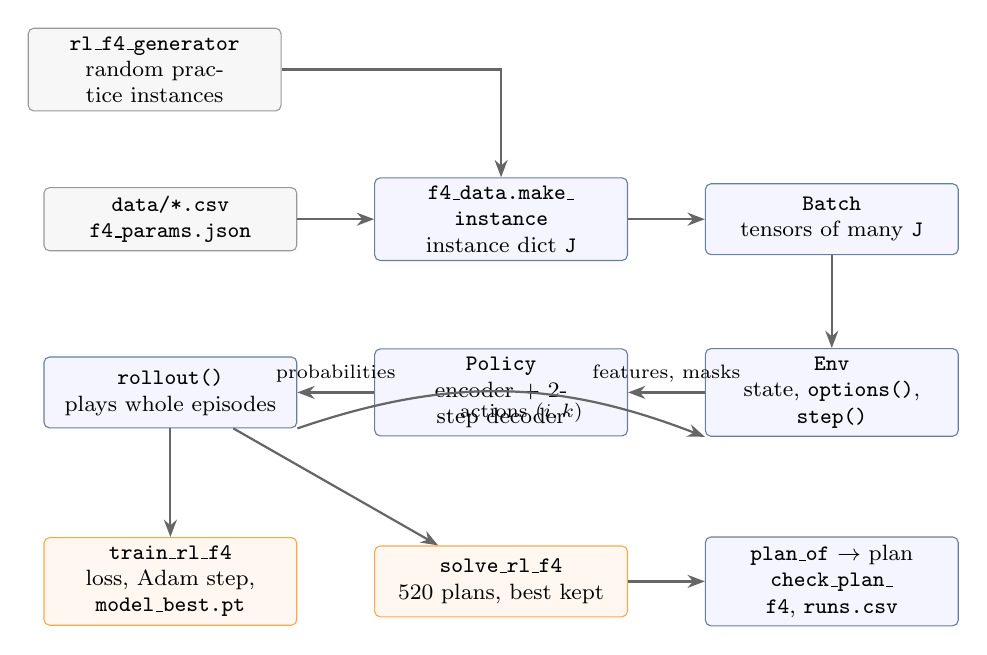
\begin{tikzpicture}[font=\footnotesize,
  box/.style={draw=headblue!70,fill=blue!4,rounded corners=2pt,align=center,minimum height=9mm,inner sep=3pt,text width=3.0cm},
  data/.style={draw=black!40,fill=black!3,rounded corners=2pt,align=center,minimum height=8mm,inner sep=3pt,text width=3.0cm},
  arr/.style={-{Stealth[length=2.2mm]},thick,draw=black!60}]
\node[data] (csv) at (0,0) {\code{data/*.csv}\\ \code{f4\_params.json}};
\node[box] (inst) at (4.2,0) {\code{f4\_data.make\_instance}\\ instance dict \code{J}};
\node[box] (batch) at (8.4,0) {\code{Batch}\\ tensors of many \code{J}};
\node[box] (env) at (8.4,-2.2) {\code{Env}\\ state, \code{options()}, \code{step()}};
\node[box] (pol) at (4.2,-2.2) {\code{Policy}\\ encoder + 2-step decoder};
\node[box] (roll) at (0,-2.2) {\code{rollout()}\\ plays whole episodes};
\node[box,fill=orange!6,draw=orange!70] (train) at (0,-4.6) {\code{train\_rl\_f4}\\ loss, Adam step, \code{model\_best.pt}};
\node[box,fill=orange!6,draw=orange!70] (solve) at (4.2,-4.6) {\code{solve\_rl\_f4}\\ 520 plans, best kept};
\node[box] (plan) at (8.4,-4.6) {\code{plan\_of} $\to$ plan\\ \code{check\_plan\_f4}, \code{runs.csv}};
\node[data] (gen) at (-0.2,1.9) {\code{rl\_f4\_generator}\\ random practice instances};
\draw[arr] (csv) -- (inst);
\draw[arr] (inst) -- (batch);
\draw[arr] (batch) -- (env);
\draw[arr] (env) -- node[above,font=\scriptsize]{features, masks} (pol);
\draw[arr] (pol) -- node[above,font=\scriptsize]{probabilities} (roll);
\draw[arr] (roll.south east) to[bend left=20] node[pos=0.55,below,font=\scriptsize]{actions $(i,k)$} (env.south west);
\draw[arr] (roll) -- (train);
\draw[arr] (roll) -- (solve);
\draw[arr] (solve) -- (plan);
\draw[arr] (gen) -| (inst);
\end{tikzpicture}
\caption{Data flow. Training uses random practice instances from the generator; solving uses the 560 test instances from \code{data/}. Both go through the same \code{Batch}, \code{Env}, \code{Policy} and \code{rollout}.}
\label{fig:flow}
\end{figure}

\subsection{Notation used everywhere}

{\small
\begin{longtable}{@{}>{\raggedright\arraybackslash}p{3.6cm}>{\raggedright\arraybackslash}p{6.4cm}>{\raggedright\arraybackslash}p{5.6cm}@{}}
\toprule
\textbf{symbol} & \textbf{meaning} & \textbf{in the code} \\
\midrule
\endhead
$I=\{1,\dots,n\}$, $i$ & cars (EVs) of the instance & index \code{i} $=0,\dots,n-1$; EV number $i+1$ \\
$F$, $f$ & fixed charging stations (12) & \code{F}, \code{n\_fcs} \\
$G$, $g$, $f(g)$ & guns (24), the station of gun $g$ & \code{G}; \code{gun\_station[g]} \\
$M$, $m$ & vans (5) & \code{M}; resource index $k=G+m$ \\
$K=G\cup M$, $k$ & all resources: $k<G$ gun, $k\ge G$ van & \code{K = G + M} \\
node $0$, node $i$ & depot, car $i$ (routing nodes) & row/column 0 and $i+1$ of \code{dN}, \code{tN} \\
$r_i$, $E_i$, $R_i$ & request minute, energy (kWh), range (km) & \code{r\_min}, \code{E\_kWh}, \code{R\_km} \\
$\tau^\Fcs_i$, $\tau^\Mcs_i$ & charging minutes at a gun / by a van & \code{tauF\_min}, \code{tauM\_min} \\
$d_{if}$, $t_{if}$ & km and minutes from car $i$ to station $f$ & \code{dEF}, \code{tEF} \\
$d_{uv}$, $t_{uv}$ & km and minutes between routing nodes & \code{dN}, \code{tN} \\
$s_i$, $\theta_i$ & segment (0 personal, 1 commercial), income & \code{segment}, \code{theta} \\
$\mu_i$, $c^D_i,c^Q_i,c^C_i,c^V_i$, $W_i$ & money sensitivity, values of time, queue tolerance & \code{mu}, \code{cD}, \code{cQ}, \code{cC}, \code{cV}, \code{W} \\
$p^\Fcs$, $p^\Mcs$ & tariffs per kWh (station, van) & \code{p\_F}, \code{p\_M} \\
$c^{EV}$, $c^\Mcs$, $c^\Fcs$ & EV km cost, van km cost, van dispatch cost & \code{c\_EV}, \code{c\_M}, \code{c\_F} \\
$\pi^\Fcs$, $\pi^\Mcs$, $\eta$ & operator energy prices, van charging efficiency & \code{pi\_F}, \code{pi\_M}, \code{eta} \\
$B$, $Q$, $\beta$, $T$ & van battery, seats, van kWh per km, period length & \code{Bk}, \code{Q}, \code{beta}, \code{T} \\
$S_i$, $C_i$ & start and completion minute of car $i$ & \code{S}, \code{C} \\
\bottomrule
\end{longtable}}

\inshort{The RL is four pieces: the data turns into tensors, the environment keeps the partial plan and says which decisions are allowed and what each costs, the network chooses, and the training and solving scripts play many episodes with it.}

%=====================================================================
\section{The problem as the MILP states it}
\label{sec:milp}

The RL solves exactly the same problem as the MILP of \code{formulation\_4.pdf}. To compare the two later (Section~\ref{sec:compare}), here is the MILP in one place. Formulation 4 has the variables and constraints of formulation 3; only the per-car coefficients $\mu_i$, $c^a_i$, $W_i$ depend on the segment.

\subsection{Decision variables}
\begin{itemize}
  \item $y_{ig}\in\{0,1\}$: car $i$ charges at gun $g$ (only guns of stations within range, $g\in G_i$);
  \item $z_{im}\in\{0,1\}$: car $i$ is served by van $m$;
  \item $x_{uvm}\in\{0,1\}$: van $m$ drives from node $u$ to node $v$ (depot $0$ / $n+1$, cars $1..n$);
  \item $u_m\in\{0,1\}$: van $m$ leaves the depot;
  \item $o_{ij}\in\{0,1\}$: car $i$ is charged before car $j$ on a shared gun;
  \item $S_i\ge0$: start of car $i$'s charging; $q^\Fcs_i\ge0$ queue at a station; $q^\Mcs_i\ge0$ wait for a van.
\end{itemize}
Short-hands: $y_i=\sum_g y_{ig}$ (station user), $z_i=\sum_m z_{im}$ (van user), $Y_{if}=\sum_{g\in G_f}y_{ig}$, $C_i=S_i+\tau^\Fcs_i y_i+\tau^\Mcs_i z_i$.

\subsection{Objective}
\begin{equation}
\begin{aligned}
\min Z=&\underbrace{\sum_i\mu_i c^{EV}\sum_f d_{if}Y_{if}}_{Z_1}
+\underbrace{c^\Mcs\sum_m\sum_{(u,v)}d_{uv}x_{uvm}}_{Z_2}
+\underbrace{c^\Fcs\sum_m u_m}_{Z_3}
+\underbrace{\pi^\Fcs\sum_i E_iy_i+\pi^\Mcs\sum_i\tfrac{E_i}{\eta}z_i}_{Z_4}\\
&+\underbrace{\sum_i\mu_iE_i\big(p^\Fcs y_i+p^\Mcs z_i\big)}_{Z_5}
+\underbrace{\sum_i\Big(c^D_i\sum_f t_{if}Y_{if}+c^Q_iq^\Fcs_i+c^C_i\tau^\Fcs_iy_i+c^V_i\big(q^\Mcs_i+\tau^\Mcs_iz_i\big)\Big)}_{Z_6}.
\end{aligned}\tag{1}
\end{equation}

\subsection{Constraints}
{\small
\begin{longtable}{@{}l>{\raggedright\arraybackslash}p{7.3cm}>{\raggedright\arraybackslash}p{6.3cm}@{}}
\toprule
no. & constraint & meaning \\
\midrule
\endhead
(2) & $\sum_{g\in G_i}y_{ig}+\sum_m z_{im}=1$ & every car gets exactly one resource \\
(3) & $S_i\ge r_i+\sum_f t_{if}Y_{if}$ & a station user starts only after driving there \\
(4) & $q^\Fcs_i+q^\Mcs_i=S_i-r_i-\sum_f t_{if}Y_{if}$ & the waiting time \\
(5) & $q^\Fcs_i\le W_iy_i$ & queue at most $W_i$ \\
(6) & $q^\Mcs_i\le Tz_i$ & only van users wait for a van \\
(7)--(8) & $S_j\ge S_i+\tau^\Fcs_i-M(3-y_{ig}-y_{jg}-o_{ij})$ and the reverse & two cars on one gun do not overlap \\
(9) & $\sum_i\tau^\Fcs_iy_{ig}\le T-\min_i(r_i+t_{if(g)})$ & gun-load cut (valid inequality, tightens the LP) \\
(10) & $\sum_iy_{ig_1}\ge\sum_iy_{ig_2}$ & symmetry: gun 1 of a station before gun 2 \\
(11)--(12) & $\sum_v x_{0vm}=u_m$, $\sum_u x_{u,n+1,m}=u_m$ & a used van leaves and returns once \\
(13)--(14) & $\sum_u x_{ujm}=z_{jm}$, $\sum_v x_{jvm}=z_{jm}$ & a van enters and leaves each of its cars once \\
(15) & $\sum_iz_{im}\le Qu_m$ & at most $Q$ cars per van \\
(16) & $\sum_i\frac{E_i}{\eta}z_{im}+\beta\sum_{(u,v)}d_{uv}x_{uvm}\le Bu_m$ & battery covers charging and driving \\
(17) & $S_j\ge t_{0j}x_{0jm}$ & the first car waits for the van to arrive \\
(18) & $S_j\ge S_i+\tau^\Mcs_i+t_{ij}-M(1-x_{ijm})$ & a van charges one car at a time, in route order \\
(19) & $S_i+\tau^\Mcs_i+t_{i,n+1}\le T+\dots(1-x_{i,n+1,m})$ & the van is back at the depot by $T$ \\
(20) & $S_i\ge r_i$ & no charging before the request \\
(21) & $C_i\le T$ & every car fully charged by $T$ \\
(22) & $u_m\ge u_{m+1}$ & symmetry: vans used in order \\
(23) & domains (binary / non-negative) & \\
\bottomrule
\end{longtable}}

For a 100-car instance this model has thousands of binary variables (one $x$ per pair of cars per van, one $o$ per pair of cars per shared gun). Gurobi needs up to 300 seconds and may still not prove optimality. The RL never builds these variables; it reaches the same kind of plan by construction.

\inshort{The MILP decides everything at once with binary variables and big-$M$ constraints; the RL will make the same decisions one at a time and check the same rules directly.}

%=====================================================================
\section{From the data files to numbers: the instance dictionary}
\label{sec:data}

Every method (MILP, RL, checker) starts from the same Python dictionary \code{J}, built by \code{common/f4\_data.py}. An instance is one file of \code{data/solomon\_data.csv} and its first $n$ cars.

\subsection{Distances, times and charging durations}

\src{../../common/f4_data.py}{61}{65}

\begin{itemize}
  \item Line 61: $k=\text{detour}\times\text{km per grid unit}=1.3\times0.2$.
  \item Line 62: road distance car--station, $d_{if}=k\,\lVert x_i-x_f\rVert$ (km).
  \item Lines 63--64: the routing nodes are the depot (node 0) and the cars (nodes $1..n$); $d_{uv}$ between all of them.
  \item Line 65: charging minutes $\tau^\Fcs_i=60E_i/P^\Fcs$ and $\tau^\Mcs_i=60E_i/P^\Mcs$ (22 kW and 30 kW).
  \item Travel minutes (line 87): $t=60\,d/v$ with speed $v=15.6$ km/h, chosen so that minutes equal grid distance (Solomon's rule).
\end{itemize}

\subsection{The customer coefficients}

Each customer's $\mu_i$, $c^a_i$ and $W_i$ are read off the straight line of its segment at its $\theta_i$:

\src{../../common/f4_params.py}{144}{145}
\src{../../common/f4_params.py}{157}{172}

In formulas, for segment $s_i$ and each quantity $x\in\{\mu,c^D,c^Q,c^C,c^V,W\}$:
\[
x_i=x^{s_i,0}+\big(x^{s_i,1}-x^{s_i,0}\big)\,\theta_i ,
\]
with the end points $x^{s,0}$, $x^{s,1}$ of \code{f4\_params.json} (lines 167--169; values of time and $W$ are kept non-negative). Line 171 picks the commercial line where \code{seg == 1} and the personal line elsewhere. These numbers are fixed before any solving starts, which is why the MILP stays linear and why the RL can treat them as data.

\subsection{What is in \code{J}}

{\small
\begin{longtable}{@{}>{\raggedright\arraybackslash}p{4.4cm}>{\raggedright\arraybackslash}p{11.4cm}@{}}
\toprule
key & content \\
\midrule
\endhead
\code{n\_ev}, \code{n\_fcs}, \code{n\_vans} & $n$, number of stations (12), vans (5) \\
\code{params} & $T$, guns per station, $\eta$, $\beta$, $B$, $Q$, costs ($c^{EV},c^\Mcs,c^\Fcs,\pi^\Fcs,\pi^\Mcs$), tariffs ($p^\Fcs,p^\Mcs$) \\
\code{ev} & per car: $E_i$, $r_i$, $R_i$, $\tau^\Fcs_i$, $\tau^\Mcs_i$, $\theta_i$, $s_i$, $\mu_i$, $c^D_i$, $c^Q_i$, $c^V_i$, $c^C_i$, $W_i$ \\
\code{d\_ev\_fcs\_km}, \code{t\_ev\_fcs\_min} & $n\times F$ matrices $d_{if}$, $t_{if}$ \\
\code{d\_nodes\_km}, \code{t\_nodes\_min} & $(n+1)\times(n+1)$ matrices $d_{uv}$, $t_{uv}$ (node 0 = depot) \\
\code{xy} & coordinates of depot, stations, cars (only the network uses them) \\
\bottomrule
\end{longtable}}

\inshort{Before anything is solved, every car is turned into numbers: where it is, when it asks, how much it needs, how far every station is, and how it feels money and time.}

%=====================================================================
\section{The environment: \code{rl\_f4\_env.py}}
\label{sec:env}

The environment is the ``game'' the policy plays. It answers three questions at every step: \emph{which decisions are allowed?}, \emph{what does each cost?}, and \emph{what does the partial plan look like after the decision?} Everything is written with PyTorch tensors so that many episodes (many instances, or many tries on one instance) run side by side; the first dimension of every tensor is the \emph{row} $b$ of the batch.

\subsection{\code{Batch}: the static data as tensors}

\src{../code/rl_f4_env.py}{53}{65}

\begin{itemize}
  \item A batch holds $B$ instances with the same $n$, stations, guns and vans (line 59 checks it), so that they fit in one tensor.
  \item Lines 62--63 number the guns: station 1 has guns 0 and 1, station 2 has guns 2 and 3, and so on. \code{gun\_station[g]} is $f(g)$; with 12 stations of 2 guns, $G=24$.
  \item Line 65: the resources are the $G$ guns followed by the $M$ vans, $K=G+M=29$. A resource index $k<G$ is a gun, $k\ge G$ is van $k-G$.
\end{itemize}

Lines 71--87 copy every number of \code{J} into tensors of shape $(B,n)$, $(B,n,F)$, $(B,n{+}1,n{+}1)$ or $(B,)$, in 64-bit floating point (so feasibility decisions agree exactly with the checker). Lines 88--99 then compute quantities that never change during an episode:

\src{../code/rl_f4_env.py}{88}{100}

\begin{itemize}
  \item \code{reach\_g}$[i,g]=\big[d_{i f(g)}\le R_i\big]$: car $i$ can reach gun $g$'s station;
  \item \code{arrive\_g}$[i,g]=r_i+t_{i f(g)}$: when car $i$ would arrive there;
  \item cost of gun $g$ for car $i$ without any queue:
  \[
  \text{\code{gun\_cost0}}[i,g]=\mu_i\big(c^{EV}d_{if(g)}+p^\Fcs E_i\big)+\pi^\Fcs E_i+c^D_it_{if(g)}+c^C_i\tau^\Fcs_i ;
  \]
  \item cost of a van for car $i$ without wait and without the van's driving:
  \[
  \text{\code{van\_cost0}}[i]=\mu_ip^\Mcs E_i+\pi^\Mcs\frac{E_i}{\eta}+c^V_i\tau^\Mcs_i ;
  \]
  \item \code{d\_back}$[i]=d_{i0}$, \code{t\_back}$[i]=t_{i0}$: from car $i$ back to the depot.
\end{itemize}
\code{gun\_cost0} and \code{van\_cost0} are the parts of the cost increase that depend only on the car and the resource type; the parts that depend on the current state (queue, van wait, van position, whether the van is new) are added in \code{options()}.

\subsection{\code{Env}: the state}

\src{../code/rl_f4_env.py}{126}{157}

{\small
\begin{longtable}{@{}>{\raggedright\arraybackslash}p{2.6cm}>{\raggedright\arraybackslash}p{1.6cm}>{\raggedright\arraybackslash}p{2.4cm}>{\raggedright\arraybackslash}p{8.6cm}@{}}
\toprule
tensor & shape & start value & meaning \\
\midrule
\endhead
\code{done} & $(B,n)$ & false & car $i$ is placed or dropped \\
\code{dropped} & $(B,n)$ & false & car $i$ could not be placed (no allowed resource left) \\
\code{gun\_free} & $(B,G)$ & 0 & $a_g$: the minute gun $g$ becomes free (completion of its last car) \\
\code{van\_pos} & $(B,M)$ & 0 & $\ell_m$: node where van $m$ is (0 = depot, $i+1$ = car $i$) \\
\code{van\_free} & $(B,M)$ & 0 & $a_m$: the minute van $m$ finishes its last car \\
\code{van\_batt} & $(B,M)$ & $B$ & $b_m$: battery left (kWh) \\
\code{van\_cnt} & $(B,M)$ & 0 & $\kappa_m$: cars served so far \\
\code{cost} & $(B,)$ & 0 & sum of the cost increases so far ($=Z$ of the partial plan) \\
\code{res}, \code{S}, \code{C}, \code{order} & $(B,n)$ & $-1$, 0, 0, $-1$ & the plan: resource, start, completion and step number of each car \\
\code{steps} & int & 0 & decisions taken \\
\bottomrule
\end{longtable}}

This is the full \textbf{state} of the decision process:
\[
s_t=\Big(P_t,\ D_t,\ (a_g)_{g\in G},\ (\ell_m,a_m,b_m,\kappa_m)_{m\in M}\Big),
\]
with $P_t$ the placed and $D_t$ the dropped cars. Everything the future depends on is in it: the cost of every remaining decision can be computed from $s_t$ alone (this is the \emph{Markov property}).

Two extra quantities are prepared once:
\begin{itemize}
  \item \code{same\_earlier[g,g']} (line 149) is true when $g'<g$ and both guns belong to the same station. It is used for the symmetry rule below.
  \item \code{cost\_scale} (lines 152--157), written $\sigma$: the average, over the cars, of their cheapest allowed option at the start. It is a ``typical cost of one car'' for this instance, used to scale features and the penalty for unplaced cars:
  \[
  \sigma=\max\Big(1,\ \frac{1}{|\{i:\exists k\}|}\sum_{i}\min_{k\text{ allowed}}\Delta Z(i,k)\Big).
  \]
\end{itemize}

\subsection{The action}

An \textbf{action} is a pair $(i,k)$: car $i$ (not yet done) goes to resource $k$. It is appended to the \emph{end} of $k$'s sequence: the end of gun $k$'s queue, or the next stop of van $k-G$'s route. The policy chooses the pair in two steps, first $i$ and then $k$ (Section~\ref{sec:network}); the environment does not care how it was chosen.

\subsection{\code{options()}: what every possible action would do}
\label{sec:options}

\code{options()} computes, for \emph{every} unplaced car $i$ and \emph{every} resource $k$ at once, the start, wait, finish, whether the pair is allowed (the \emph{mask}), and the cost increase $\Delta Z(i,k)$. The result has shape $(B,n,K)$.

\src{../code/rl_f4_env.py}{160}{195}

\paragraph{Guns (lines 165--172).} If car $i$ is sent to gun $g$:
\begin{align*}
S_i&=\max\big(r_i+t_{if(g)},\ a_g\big) &&\text{arrive, or wait until the gun is free (line 166)}\\
q^\Fcs_i&=S_i-r_i-t_{if(g)} &&\text{queue (line 167)}\\
C_i&=S_i+\tau^\Fcs_i &&\text{finish (line 168)}
\end{align*}
The pair is \textbf{allowed} (line 170) if all four hold:
\[
d_{if(g)}\le R_i,\qquad q^\Fcs_i\le W_i,\qquad C_i\le T,
\]
and no earlier gun of the same station is free at the same minute.
The last condition (lines 169, 171) is the \emph{symmetry rule}: two idle guns of one station are identical, so only the first is offered. The cost increase (line 172) is
\[
\Delta Z(i,g)=\text{\code{gun\_cost0}}[i,g]+c^Q_i\,q^\Fcs_i .
\]

\paragraph{Vans (lines 174--191).} If car $i$ is the next stop of van $m$, which is at node $\ell_m$ and free at $a_m$:
\begin{align*}
S_i&=\max\big(r_i,\ a_m+t_{\ell_m i}\big) &&\text{the van drives over; the car must have requested (line 179)}\\
q^\Mcs_i&=S_i-r_i &&\text{wait for the van (line 180)}\\
C_i&=S_i+\tau^\Mcs_i &&\text{finish (line 181)}\\
\text{need}_{im}&=\frac{E_i}{\eta}+\beta\big(d_{\ell_m i}+d_{i0}\big) &&\text{energy to charge $i$, drive there and get home (line 182)}
\end{align*}
The pair is \textbf{allowed} (lines 185--187) if all four hold:
\[
\kappa_m<Q,\qquad \text{need}_{im}\le b_m,\qquad C_i+t_{i0}\le T,
\]
and the van is already in use ($\kappa_m>0$) or is the first unused van.
The last condition is again a symmetry rule: unused vans are identical (all at the depot, full battery), so only the first is offered (lines 183--184). The cost increase (lines 188--191) is
\[
\Delta Z(i,m)=\text{\code{van\_cost0}}[i]+c^\Mcs\big(d_{\ell_m i}+d_{i0}-d_{\ell_m0}\big)+c^\Fcs\,[\kappa_m=0]+c^V_i\,q^\Mcs_i .
\]
The van-km term is the \emph{extra} driving: before, the van's route ended $\ell_m\to0$; now it ends $\ell_m\to i\to0$. The dispatch cost $c^\Fcs$ is charged when a van gets its first car.

\paragraph{Line 192.} Cars that are already done get no allowed resource. The returned dictionary keeps the full $(B,n,K)$ tensors (\code{feas}, \code{finish}, \code{dz}) and the gun and van parts of start and wait separately (they are read later only for the chosen car, which saves memory).

\subsection{\code{drop\_dead()} and \code{step()}: what happens after a decision}

\src{../code/rl_f4_env.py}{201}{235}

\textbf{\code{drop\_dead}} (lines 201--207): a car with no allowed resource is marked done \emph{and} dropped. It can never become placeable again (Proposition~\ref{prop:dead}), so waiting would only waste steps.

\textbf{\code{step}} (lines 209--235) applies action $(i,k)$ in every active row:
\begin{itemize}
  \item lines 216--218: read the start and finish computed by \code{options()};
  \item line 219: \code{cost} $\leftarrow$ \code{cost} $+\Delta Z(i,k)$;
  \item lines 220--223: record the plan (resource, $S_i$, $C_i$, step number) and mark the car done;
  \item gun (line 226): $a_g\leftarrow C_i$;
  \item van (lines 229--234):
  \[
  b_m\leftarrow b_m-\frac{E_i}{\eta}-\beta\,d_{\ell_m i},\qquad \ell_m\leftarrow i,\qquad a_m\leftarrow C_i,\qquad \kappa_m\leftarrow\kappa_m+1 .
  \]
  The way home is \emph{not} subtracted from the battery yet; it was only checked in the mask, and it will be checked again from the new position for the next car.
\end{itemize}
The environment is \textbf{deterministic}: the same actions always give the same plan.

\textbf{End of an episode} (\code{finished()}, line 237): when every car is done (placed or dropped).

\subsection{What the network sees: the features}
\label{sec:features}

The network never sees the raw tensors; \code{rl\_f4\_env.py} turns the state into scaled numbers.

\paragraph{Static features} (lines 245--274), computed once per instance:

\src{../code/rl_f4_env.py}{263}{273}

{\small
\begin{longtable}{@{}r>{\raggedright\arraybackslash}p{6.6cm}>{\raggedright\arraybackslash}p{8.0cm}@{}}
\toprule
\# & car feature & formula \\
\midrule
\endhead
1--2 & position relative to the depot & $(x_i-x_0)/\text{scale}$, one of 8 map symmetries \\
3 & request time & $r_i/T$ \\
4--5 & charging times & $\tau^\Fcs_i/T$, $\tau^\Mcs_i/T$ \\
6 & queue tolerance & $W_i/T$ \\
7 & income & $\theta_i$ \\
8 & energy & $E_i/B$ \\
9 & stranded & $1$ if no station is within range \\
10 & share of reachable stations & $|F_i|/F$ \\
11 & time to the nearest reachable station & $\min_{f\in F_i}t_{if}/T$ \\
12 & time back to the depot & $t_{i0}/T$ \\
13 & range relative to the city & $R_i/\max d_{if}$ \\
14 & cheapest gun cost & $\min_g\text{\code{gun\_cost0}}[i,g]/\sigma$ \\
15 & van cost & $\text{\code{van\_cost0}}[i]/\sigma$ \\
16 & how late a van may come & $(T-r_i-\tau^\Mcs_i-t_{i0})/T$ \\
17 & \textbf{commercial} (new in f4) & $s_i\in\{0,1\}$ \\
18 & \textbf{money sensitivity} (new) & $\mu_i/2$ \\
19 & \textbf{cost of queueing one charge} (new) & $c^Q_i\tau^\Fcs_i/\sigma$ \\
\bottomrule
\end{longtable}}
Each station has 4 features (position, guns/2, share of cars that can reach it); the depot has 4 (seats per car $QM/n$, guns per car $G/n$, $\log T/8$, $n/100$).

\paragraph{Dynamic features}, recomputed at every step from \code{options()} and the state:
\begin{itemize}
  \item \textbf{global} (4, lines 276--281): share of cars done, mean gun busy time $/T$, share of vans in use, mean battery left $/B$;
  \item \textbf{per car} $\varphi_i$ (7, lines 283--314): share of resources still allowed; cheapest $\Delta Z/\sigma$; \emph{regret} = (second-cheapest $-$ cheapest)$/\sigma$; earliest finish $/T$; (cheapest gun $-$ cheapest van)$/\sigma$; request time relative to the earliest open request; place in the queue of open requests (0 = next, 1 = last; ties broken by higher $c^Q$);
  \item \textbf{per resource} $\rho_k$ (6, lines 316--325): free time $/T$, van flag, battery left $/B$, seats used $/Q$, in use, time back to the depot $/T$ (van-only entries are 0 for guns);
  \item \textbf{per pair} (6, lines 327--344), only for the chosen car $i$: $\Delta Z(i,k)/\sigma$, its excess over the cheapest option, wait $/T$, finish $/T$, battery left after serving $i$, van flag; all zero for masked resources.
\end{itemize}

\subsection{\code{GreedyRule}: the simple rule}

\src{../code/rl_f4_env.py}{348}{365}

The order is built with three stable sorts (lines 356--358): first by $c^Q$ (highest first), then by request time, then stranded cars first, so the final order is \emph{stranded first, then earliest request, then the customer who hates queueing most}. At each step the first car in that order that is not done takes its cheapest allowed resource (lines 363--365). This is the MILP's own starting plan (\code{greedy\_f4}); in the RL it is the teacher of the warm-up and the yardstick of the validation.

\subsection{\code{plan\_of}: from an episode to a plan}

\src{../code/rl_f4_env.py}{423}{439}

Lines 423--438 turn the recorded resources into the plan format shared with the MILP: ``FCS$f$-gun$g$'' for station users, ``van$v$'' for van users (vans in use numbered $1,2,\dots$ like the MILP), and each van's route $[0,\dots,0]$ in the order the cars were added. Lines 395--422 (not shown) handle dropped cars: they are appended to whichever resource finishes them earliest, \emph{ignoring} the rule they break, so the plan is complete; the checker then lists the violation and the plan is reported as \code{invalid\_plan}.

\inshort{The environment keeps the partial plan (when each gun is free; where each van is, when it is free, how much battery and how many seats it has left). For every possible next decision it computes the start time, whether any rule is broken, and the exact cost increase. Applying a decision updates the plan and adds the cost.}

%=====================================================================
\section{The reward function}
\label{sec:reward}

\subsection{Definition}

In RL language, after every action the environment gives a \emph{reward}; the agent tries to make the total reward of an episode (the \emph{return}) as large as possible. Here the reward of action $(i_t,k_t)$ is minus the increase of the objective:
\[
\boxed{\;r_t=-\Delta Z(i_t,k_t)\;}
\qquad\text{with}\qquad
\Delta Z(i,g)=\underbrace{\mu_ic^{EV}d_{if(g)}}_{Z_1}+\underbrace{\pi^\Fcs E_i}_{Z_4}+\underbrace{\mu_ip^\Fcs E_i}_{Z_5}+\underbrace{c^D_it_{if(g)}+c^Q_iq^\Fcs_i+c^C_i\tau^\Fcs_i}_{Z_6}
\]
for a gun, and for a van
\[
\Delta Z(i,m)=\underbrace{c^\Mcs\big(d_{\ell_mi}+d_{i0}-d_{\ell_m0}\big)}_{Z_2}+\underbrace{c^\Fcs[\kappa_m=0]}_{Z_3}+\underbrace{\pi^\Mcs\tfrac{E_i}{\eta}}_{Z_4}+\underbrace{\mu_ip^\Mcs E_i}_{Z_5}+\underbrace{c^V_i\big(q^\Mcs_i+\tau^\Mcs_i\big)}_{Z_6}.
\]
Each part is labelled with the term of the MILP objective (1) it belongs to. There is no discount: the return of an episode is $\sum_tr_t$.

In the code there is no variable called ``reward''. \code{options()} computes $\Delta Z$ for every pair (\code{dz}, lines 172 and 188--191 of \code{rl\_f4\_env.py}), and \code{step()} adds the chosen one to \code{env.cost} (line 219). At the end of an episode, \code{env.cost} $=\sum_t\Delta Z_t=-\sum_tr_t$.

\subsection{The rewards add up exactly to the MILP objective}

\begin{proposition}\label{prop:sum}
If an episode places every car, $\sum_t\Delta Z(i_t,k_t)=Z$ of the resulting plan, with $Z$ as in (1).
\end{proposition}
\begin{proof}
$Z_1$, $Z_4$, $Z_5$, $Z_6$ are sums over cars, and each car's terms are added exactly once, when it is placed. $Z_3$: $c^\Fcs$ is added when a van gets its first car ($\kappa_m=0$), so once per used van. $Z_2$: a van with route $0\to i_1\to i_2\to\dots\to i_k\to0$ adds
\[
c^\Mcs\big[(d_{0i_1}+d_{i_10}-d_{00})+(d_{i_1i_2}+d_{i_20}-d_{i_10})+\dots+(d_{i_{k-1}i_k}+d_{i_k0}-d_{i_{k-1}0})\big].
\]
Each $d_{i_j0}$ is added once and subtracted once at the next stop, except the last; with $d_{00}=0$ the sum is $c^\Mcs(d_{0i_1}+d_{i_1i_2}+\dots+d_{i_k0})$, the route length times $c^\Mcs$.
\end{proof}
Section~\ref{sec:trace} checks this on a real episode: the simulator's sum and the independent checker's $Z$ agree to the last paisa.

\subsection{What the training actually minimises: the penalised cost}

If a car is dropped, the plan breaks the hard rule ``every car is served''. Training therefore uses
\[
\tilde c=Z+\lambda\,\sigma\,|D|,\qquad \lambda=10\ \ (\text{\code{drop\_penalty}}),
\]
where $|D|$ is the number of dropped cars and $\sigma$ the instance's typical cost per car (\code{cost\_scale}). A dropped car therefore costs as much as about ten ordinary cars, so the policy learns that leaving a car without a charger is never worth it. Measuring the penalty in units of $\sigma$ makes it comparable between cheap and expensive instances. This is \code{penalised\_cost} (lines 240--242).

When the best of several plans is chosen (validation, solving), the order is \emph{fewest dropped cars first, then lowest $Z$}: the code uses the key $10^{12}|D|+Z$ (Section~\ref{sec:solve}).

\subsection{Why the step costs matter even though training uses only the total}

REINFORCE (Section~\ref{sec:training}) only needs the total $\tilde c$ of each episode. The per-step $\Delta Z$ is still essential:
\begin{itemize}
  \item it is how the total is computed, exactly, without a separate evaluation;
  \item it feeds the features: the cheapest option of each car, its regret, and the pair feature $\Delta Z(i,k)/\sigma$ tell the network directly what each choice costs now;
  \item it is the teacher's criterion: the greedy rule picks the smallest $\Delta Z$.
\end{itemize}

\subsection{Three more facts that make the design correct}

\begin{proposition}[Earliest start is optimal]\label{prop:timing}
Fix which resource serves each car and the order on every gun and van. If some start times satisfy all rules, the earliest-start times computed by \code{options()} satisfy them too, and give a $Z$ that is not higher.
\end{proposition}
\begin{proof}[Idea of the proof]
With the order fixed, the rules on start times are lower bounds ($S_i\ge r_i+t_{if}$, $S_j\ge C_i$ on a gun, $S_j\ge C_i+t_{ij}$ on a van) and upper bounds ($q^\Fcs_i\le W_i$, $C_i\le T$, back by $T$). The earliest schedule meets every lower bound with the smallest possible times, so it also meets every upper bound that any other schedule meets. $Z$ depends on start times only through $c^Q_iq^\Fcs_i$ and $c^V_iq^\Mcs_i$, which grow with later starts.
\end{proof}

\begin{proposition}[No plan is out of reach]\label{prop:complete}
Every feasible plan of the MILP can be produced by some sequence of allowed actions (up to swapping identical guns or vans), with a cost not higher.
\end{proposition}
\begin{proof}[Idea of the proof]
Add the cars in the order of their start times in that plan. Each resource's sequence is rebuilt in its own order, the earliest start times are not later than the plan's, so queue, deadline and return rules hold; the van battery check holds because by the triangle inequality the rest of the route home is at least $d_{i0}$ long.
\end{proof}

\begin{proposition}[A dead car stays dead]\label{prop:dead}
If a car has no allowed resource now, it has none later.
\end{proposition}
\begin{proof}[Idea of the proof]
Gun free times only grow (so queues and finishes only grow); van seats only fill; a van that moves on is, by the triangle inequality, no earlier and no closer in energy to any car; unused vans do not change.
\end{proof}

Together: the action space loses no plan (Proposition~\ref{prop:complete}), the timing is the best possible (Proposition~\ref{prop:timing}), the reward is exactly the objective (Proposition~\ref{prop:sum}), and dropping dead cars early loses nothing (Proposition~\ref{prop:dead}). The full proofs are in \code{RL\_implementation\_report.pdf}, Section 6.

\inshort{The reward of each decision is minus the exact increase of the MILP objective it causes. The rewards of an episode add up to $-Z$; training adds a large penalty for every car left without a charger.}

%=====================================================================
\section{The RL side by side with the MILP formulation}
\label{sec:compare}

\subsection{Where each MILP variable lives in the RL}

\begin{table}[H]
\centering\small
\caption{Every MILP decision variable and how the same decision appears in an RL episode.}
\begin{tabularx}{\textwidth}{@{}l>{\raggedright\arraybackslash}X>{\raggedright\arraybackslash}p{4.6cm}@{}}
\toprule
MILP & RL equivalent & code \\
\midrule
$y_{ig}=1$ & action $(i,g)$ with $g<G$ was taken & \code{env.res[i] == g} \\
$z_{im}=1$ & action $(i,G+m)$ was taken & \code{env.res[i] == G+m} \\
$x_{uvm}=1$ & cars $u$ and $v$ were added to van $m$ one after the other (or $u=0$ for the first, $v=n+1$ after the last) & route in \code{plan\_of}, sorted by \code{order} \\
$u_m=1$ & van $m$ got at least one car & \code{van\_cnt[m] > 0} \\
$o_{ij}=1$ & on a shared gun, car $i$ was added before car $j$ & \code{order[i] < order[j]} \\
$S_i$ & earliest start, computed when $i$ is added & \code{env.S[i]} (from \code{start\_g} / \code{start\_v}) \\
$q^\Fcs_i$, $q^\Mcs_i$ & queue / van wait at that moment & \code{wait\_g}, \code{wait\_v} \\
$C_i$ & $S_i$ plus the charging time & \code{env.C[i]} \\
\bottomrule
\end{tabularx}
\end{table}

The RL never creates these variables; they are \emph{recovered} from the order and the choices of the episode. The MILP has one binary per possible pair of cars per van and per shared gun (thousands); the RL instead makes $n$ decisions, each among at most $n\times K$ pairs.

\subsection{Where each MILP constraint lives in the RL}

{\small
\begin{longtable}{@{}l>{\raggedright\arraybackslash}p{4.2cm}>{\raggedright\arraybackslash}p{10.0cm}@{}}
\toprule
no. & MILP constraint & how the RL guarantees it \\
\midrule
\endhead
(2) & one resource per car & each car is chosen once and then marked \code{done}; masks exclude done cars (\code{options}, line 192) \\
(3), (20) & start after arrival / request & by construction: $S_i=\max(r_i+t_{if},a_g)$ or $\max(r_i,a_m+t_{\ell_mi})$ \\
(4) & definition of the waits & computed directly: \code{wait\_g}, \code{wait\_v} \\
(5) & queue $\le W_i$ & gun mask: \code{wait\_g <= W} (line 170) \\
(6) & only van users wait for vans & automatic: a station user has no van wait \\
(7)--(8) & no overlap on a gun & by construction: a car is added at the end of the gun's queue and starts after $a_g$, the completion of the previous car \\
(9) & gun-load cut & not needed: it is a \emph{valid inequality} (implied by the others); the MILP has it only to help Gurobi's bounds \\
(10) & gun symmetry & symmetry mask: of identical idle guns of one station only the first is offered (lines 169, 171) \\
(11)--(14) & route structure (leave, visit once, return) & by construction: a van's cars form one sequence from the depot; the return is implied \\
(15) & at most $Q$ cars & van mask: $\kappa_m<Q$ (line 185) \\
(16) & battery & van mask: $E_i/\eta+\beta(d_{\ell_mi}+d_{i0})\le b_m$ (lines 182, 186); $b_m$ decreases after each car \\
(17)--(18) & van timing, one car at a time & by construction: $S_i\ge a_m+t_{\ell_mi}$, where $a_m$ is the completion of the van's previous car \\
(19) & back at the depot by $T$ & van mask: $C_i+t_{i0}\le T$ (line 187); checked for the newest last car each time \\
(21) & charged by $T$ & masks: $C_i\le T$ for guns (line 170); for vans implied by (19) \\
(22) & van symmetry & symmetry mask: only the first unused van is offered (lines 183--185) \\
(23) & domains & automatic \\
\bottomrule
\end{longtable}}

\textbf{One difference in what ``infeasible'' means.} The MILP either finds a plan satisfying all rules or reports none. The RL always produces a complete assignment, but if a car was dropped, \code{plan\_of} puts it on the resource that finishes it earliest and breaks a rule; the checker marks the plan invalid. So ``no valid plan'' is reported the same way for both, and an invalid RL plan is never counted as a solution.

\subsection{The objective}

Proposition~\ref{prop:sum} shows that the sum of the RL's step costs is exactly $Z$ of (1). The split of the six terms across the steps is in the boxed formulas of Section~\ref{sec:reward}. In practice the RL's $Z$ and the checker's $Z$ are compared for every solved instance (\code{solve\_rl\_f4.py}, line 130), and a warning is written if they differ by more than $10^{-6}$ relative; in the server run this warning appears in none of the 31 RL runs ($31\times560$ instances).

\subsection{What each method can and cannot do}

\begin{table}[H]
\centering\small
\begin{tabularx}{\textwidth}{@{}>{\raggedright\arraybackslash}p{3.4cm}>{\raggedright\arraybackslash}X>{\raggedright\arraybackslash}X@{}}
\toprule
 & MILP & RL \\
\midrule
how decisions are made & all together, by branch and bound over the binary variables & one at a time; earlier decisions are never changed \\
timing & optimised together with everything else & earliest start (optimal for the chosen orders, Proposition~\ref{prop:timing}) \\
rules & constraints (2)--(23), with big-$M$ terms & masks + construction (table above) \\
quality guarantee & proven optimal, or a known gap & none; judged against the MILP \\
time per instance & seconds to 300 s & about 0.1 s (520 tries) \\
when it fails & no plan found in time & a car left without allowed resource \\
learning & none; each instance from scratch & trained once on random instances, reused \\
\bottomrule
\end{tabularx}
\end{table}

\inshort{Every MILP rule is either a mask (range, queue limit, seats, battery, deadline, back by $T$), a consequence of adding cars at the end of sequences with earliest start times (no overlap, route structure, van timing), or not needed (the gun-load cut). The rewards add up to exactly the same $Z$.}

%=====================================================================
\section{The policy network: \code{rl\_f4\_model.py}}
\label{sec:network}

The policy $p_\phi(i,k\mid s)$ gives a probability to every allowed action; $\phi$ are its 765\,858 learned weights. It has an \emph{encoder}, run once per instance, and a two-step \emph{decoder}, run once per decision.

\subsection{The layers}

\src{../code/rl_f4_model.py}{42}{63}

\begin{table}[H]
\centering\small
\caption{The layers and their number of weights (\code{d} = 128, 8 heads, 3 encoder layers, feed-forward 512).}
\begin{tabular}{@{}llr@{}}
\toprule
layer & role & weights \\
\midrule
\code{ev\_in}, \code{st\_in}, \code{dep\_in} & 19 / 4 / 4 input features $\to$ 128 & 3\,840 \\
\code{encoder} (3 Transformer layers), \code{norm} & self-attention among all nodes & 595\,072 \\
\code{ctx} & context of step 1 & 33\,408 \\
\code{gq}, \code{gk}, \code{gv}, \code{go} & glimpse over the open cars & 65\,536 \\
\code{ev\_key}, \code{ev\_dyn} & car scores of step 1 & 16\,673 \\
\code{res\_q}, \code{res\_key} & query and keys of step 2 & 49\,280 \\
\code{gun\_dyn}, \code{van\_dyn}, \code{pair\_dyn} & resource state and pair features & 2\,049 \\
\midrule
total & & 765\,858 \\
\bottomrule
\end{tabular}
\end{table}

\subsection{Encoder}

\src{../code/rl_f4_model.py}{66}{70}

Each node gets a linear embedding of its features: $h^{(0)}_i=W_{EV}x_i+b$ for cars, similarly for stations and the depot (line 67). The $n+F+1$ vectors then pass through 3 Transformer layers (line 68). One layer does, for every node $v$:
\[
\tilde h_v=h_v+\mathrm{MHA}\big(\mathrm{LN}(h_v),\ \{\mathrm{LN}(h_u)\}_u\big),\qquad
h'_v=\tilde h_v+\mathrm{FF}\big(\mathrm{LN}(\tilde h_v)\big),
\]
where LN is layer normalisation, FF a two-layer network ($128\to512\to128$, ReLU) and MHA multi-head self-attention: with 8 heads, head $j$ computes
\[
\alpha_{vu}=\mathrm{softmax}_u\Big(\frac{(W^Q_jh_v)^\top(W^K_jh_u)}{\sqrt{16}}\Big),\qquad \text{head}_j(v)=\sum_u\alpha_{vu}W^V_jh_u ,
\]
and the 8 heads are joined and projected back to 128 numbers. In words: every node looks at every other node and takes a weighted average of what it sees; the weights are learned. Because there is no position information, the order in which the cars are listed does not matter, and the same weights work for any $n$. The output (line 70) is a vector $h_i$ per car, $h_f$ per station and $h_0$ for the depot.

\subsection{Precomputation}

\src{../code/rl_f4_model.py}{77}{86}

The projections that depend only on the embeddings are computed once per episode batch, not at every step: glimpse keys and values of the cars ($K$, $V$), the car keys for the pointer ($W_{\text{key}}h_i$), and the resource keys of stations and of all nodes (a van at node $u$ uses $W_{\text{rkey}}h_u$).

\subsection{Decoder step 1: which car?}

\src{../code/rl_f4_model.py}{89}{99}

\begin{enumerate}
  \item Lines 92--93: mean embedding of the open cars, $\bar h=\frac{1}{|\text{open}|}\sum_{i\ \text{open}}h_i$.
  \item Line 94: context $q=W_{\text{ctx}}[\bar h;\ h_0;\ \text{4 global features}]$.
  \item Lines 95--97: \emph{glimpse}: one multi-head attention from $q$ over the open cars (closed and masked cars get weight 0), giving $g$.
  \item Line 98: score of car $i$:
  \[
  u_i=\frac{(W_{\text{key}}h_i)^\top g}{\sqrt{128}}+\mathrm{MLP}(\varphi_i),
  \]
  where $\varphi_i$ are the 7 dynamic features of car $i$ (Section~\ref{sec:features}) and the MLP has one hidden layer of 32.
  \item Line 99: clip and mask: $u_i\leftarrow10\tanh(u_i)$, and $-\infty$ for cars with no allowed resource. Then $p(i)=\mathrm{softmax}(u)_i$.
\end{enumerate}

\subsection{Decoder step 2: which gun or van?}

\src{../code/rl_f4_model.py}{101}{113}

For the chosen car $i$:
\begin{enumerate}
  \item Line 104: query $q_i=W_R[h_i;\ g]$ (the car's embedding and the glimpse).
  \item Lines 108--111: key of each resource = base embedding + its current state $\rho_k$ (6 features):
  \[
  \text{key}_g=W_{\text{rkey}}h_{f(g)}+W_{\text{gun}}\rho_g,\qquad \text{key}_m=W_{\text{rkey}}h_{\ell_m}+W_{\text{van}}\rho_m .
  \]
  A gun is represented by its station; a van by the node where it currently is (the depot or its last car), which changes as the van moves.
  \item Line 112: score $v_k=\text{key}_k^\top q_i/\sqrt{128}+\mathrm{MLP}(\text{pair features of }(i,k))$; the pair features contain the exact $\Delta Z(i,k)$, wait and finish.
  \item Line 113: clip ($10\tanh$), mask the resources not allowed for car $i$, softmax: $p(k\mid i)$.
\end{enumerate}

The probability of the action is $p(i,k)=p(i)\,p(k\mid i)$.

\subsection{The episode loop: \code{rollout()}}

\src{../code/rl_f4_model.py}{123}{156}

This is the loop that plays an episode (for all rows at once):
\begin{enumerate}
  \item line 134: \code{env.options()} (allowed pairs and costs);
  \item line 135: drop cars with no allowed pair;
  \item lines 136--138: stop when every row is finished;
  \item line 139: car mask = cars with at least one allowed resource;
  \item line 141: if a teacher is given (imitation, active search), get its action;
  \item lines 142--145: step 1, choose $i$: sampled from $p(i)$, or the most likely one (greedy), or the teacher's;
  \item lines 146--152: step 2, choose $k$ the same way;
  \item lines 153--154: add $\log p(i)+\log p(k\mid i)$ to the episode's log-probability;
  \item line 155: \code{env.step} applies the action.
\end{enumerate}
It returns $\log p_\phi(\pi)=\sum_t\big[\log p(i_t)+\log p(k_t\mid i_t)\big]$, the log-probability of the whole plan; the plan and its cost are in \code{env}. Rows that are already finished take a dummy action that is not counted (lines 140, 148, 154).

\inshort{The encoder turns the instance into one vector per car, station and depot. At every step the decoder scores the open cars, picks one, then scores every gun and van for that car and picks one. The scores combine the learned vectors with the exact current costs and waits, and forbidden choices get probability zero.}

%=====================================================================
\section{Training: \code{rl\_f4\_generator.py} and \code{train\_rl\_f4.py}}
\label{sec:training}

\subsection{Practice instances}
\label{sec:generator}

The policy never trains on the 56 test files. \code{Generator.sample} makes a new random instance for every training episode, with the dataset's rules:

\src{../code/rl_f4_generator.py}{102}{137}

\begin{itemize}
  \item lines 105--107: a random Solomon class; its template gives $T$, depot, city area, stations, guns, costs and fleet;
  \item lines 110--118: positions: random (R), Gaussian clusters (C) or half and half (RC);
  \item line 119: 12 stations at $k$-means centres of the customers;
  \item line 121: $T$ varied by $\pm15$\,\%;
  \item lines 122--123: energies 10--40 kWh; lines 124--129: ranges 5--40 km, 15\,\% stranded;
  \item line 130: request times (a share at 0, the rest from a Beta distribution);
  \item lines 131--133: \textbf{segment} (commercial with probability 0.70) and \textbf{income} $\theta$ from the Beta of its segment;
  \item line 135: \code{make\_instance}, the same function as for the test data, so $\mu_i$, $c^a_i$, $W_i$ follow the same lines.
\end{itemize}
With \code{--set} (experiments) the generator uses the changed parameters and fleet, so a retrained model practises on the variant.

\subsection{Phase 1: imitation warm-up (first 500 batches)}

\src{../code/train_rl_f4.py}{129}{144}

32 practice instances with the same random $n$ (lines 132--134), each with a random map symmetry (line 136). The greedy rule plays every episode (\code{teacher=GreedyRule(env)}, line 138), and \code{rollout} returns the log-probability that the \emph{policy} gives to the rule's actions. The loss is the average negative log-likelihood per decision:
\[
\mathcal L_{\text{IL}}(\phi)=-\frac{1}{B}\sum_{b=1}^{B}\frac1n\sum_t\log p_\phi\big(a^{\text{rule}}_{b,t}\mid s_{b,t}\big)\qquad(\text{line 139}).
\]
Minimising it makes the rule's choices more likely. Then (lines 140--143): gradients, gradient-norm clipping at 1.0, one Adam step.

\subsection{Phase 2: REINFORCE with a shared baseline}

\src{../code/train_rl_f4.py}{147}{166}

\paragraph{What we want.} Make the expected cost of a plan built by the policy as small as possible:
\[
J(\phi)=\mathbb E_{x}\ \mathbb E_{\pi\sim p_\phi(\cdot\mid x)}\big[\tilde c(\pi)\big].
\]

\paragraph{The gradient (log-derivative trick).} Since $\nabla p=p\,\nabla\log p$,
\[
\nabla_\phi\,\mathbb E_\pi[\tilde c(\pi)]=\sum_\pi\tilde c(\pi)\,\nabla_\phi p_\phi(\pi)=\mathbb E_\pi\big[\tilde c(\pi)\,\nabla_\phi\log p_\phi(\pi)\big],
\]
and for any number $b$ that does not depend on the sampled $\pi$, $\mathbb E_\pi[b\,\nabla\log p_\phi(\pi)]=b\,\nabla\sum_\pi p_\phi(\pi)=0$, so
\[
\nabla_\phi J=\mathbb E\big[(\tilde c(\pi)-b)\,\nabla_\phi\log p_\phi(\pi)\big].
\]
$b$ is the \emph{baseline}: it does not change the average gradient, but a good $b$ makes the estimate much less noisy.

\paragraph{The estimate in the code.}
\begin{enumerate}
  \item Lines 148--153: $B=32$ practice instances of one random $n$; the encoder runs once per instance; the embeddings are copied $S=8$ times (line 154).
  \item Lines 155--156: $B\times S=256$ episodes are played by \emph{sampling}; \code{logp} holds $\log p_\phi(\pi_{bj})$.
  \item Line 157: penalised costs $\tilde c_{bj}$, shape $(B,S)$.
  \item Line 158: \textbf{shared baseline} (POMO): the mean of the 8 tries of the same instance, $\bar c_b=\frac18\sum_j\tilde c_{bj}$.
  \item Line 159: \textbf{advantage}, relative to that mean: $A_{bj}=(\tilde c_{bj}-\bar c_b)/\bar c_b$.
  \item Line 160: $\mathcal L_{\text{RL}}=\frac{1}{BS}\sum_{b,j}A_{bj}\log p_\phi(\pi_{bj})$. Its gradient is the estimate above (divided by $\bar c_b$).
  \item Lines 161--164: gradient, clipping, Adam step.
\end{enumerate}
\textbf{Effect.} A try that was cheaper than the average of its instance has $A<0$; the gradient step \emph{raises} the probability of all its actions. A dearer try has $A>0$; its actions become less likely. Over many batches the policy moves towards cheap plans.

Why divide by $\bar c_b$: $Z$ differs by orders of magnitude between classes and sizes; a relative advantage gives every instance the same weight. Why 8 tries of the same instance: the average of the other tries is a very good estimate of ``what the policy usually achieves on this instance'', without training a second network (critic).

\subsection{Learning rate, validation, stopping, saving}

\src{../code/train_rl_f4.py}{327}{369}

\begin{itemize}
  \item Lines 328--332: learning rate $10^{-4}$ during the warm-up, $2\times10^{-5}$ afterwards, both multiplied by $0.9998^{\text{epoch}}$.
  \item Lines 335--342: an epoch is 50 batches; the first 500 batches of a run are imitation batches, the rest REINFORCE.
  \item Lines 343--350: a failed batch is logged and skipped; 20 failures in a row stop the run.
  \item Line 353: \textbf{validation}: on 72 fixed random instances ($n=20,50,100$, 24 each), the policy's greedy plan is compared with the greedy rule's plan; the score is the mean of $\tilde c_{\text{policy}}/\tilde c_{\text{rule}}$ (below 1 = better than the rule).
  \item Lines 359--366: a better score resets the ``epochs without improvement'' counter; after epoch 200 every REINFORCE epoch without improvement increases it.
  \item Lines 367--369: \code{model\_last.pt} after every epoch; \code{model\_best.pt} whenever the score improves. Solving uses \code{model\_best.pt}.
  \item Stopping (line 327 and \code{early\_stop}, lines 321--322): at 500 epochs, after 8 hours, or after 10 epochs without improvement once epoch 200 is passed.
\end{itemize}
The baseline model of the server run: untrained score 3.57, after one warm-up epoch 1.17, best 0.969 at epoch 180, stopped at epoch 210 after 39 minutes on the RTX 4090.

\inshort{Training first copies the greedy rule, then plays each practice instance 8 times and makes the cheaper-than-average tries more likely. The best network on fixed validation instances is kept.}

%=====================================================================
\section{Solving a test instance: \code{solve\_rl\_f4.py}}
\label{sec:solve}

\src{../code/solve_rl_f4.py}{81}{103}

\begin{enumerate}
  \item Line 84: one instance becomes a batch of size 1.
  \item Lines 85--89: $A=8$ map symmetries. The encoder runs once per symmetry (line 89): the 8 rotated or mirrored copies of the map give the network 8 different inputs for the same instance (distances do not change, so every plan is valid for all of them).
  \item Lines 86--91: for each symmetry, \code{per} $=1+64$ episodes: the first one \emph{greedy} (always the most likely action), the other 64 \emph{sampled}. In total $8\times65=520$ episodes.
  \item Lines 93--96: the episodes are played in chunks of up to 1\,040 at once (memory); every chunk is a call of \code{rollout}.
  \item Lines 97--102: the best episode is kept, by the key $10^{12}\times(\text{dropped cars})+Z$, i.e.\ fewest dropped cars first, then lowest $Z$; \code{plan\_of} turns it into a plan.
\end{enumerate}

\code{run\_one} (lines 111--150) then:
\begin{itemize}
  \item scores the plan with \code{results\_io\_f4.evaluate}, which calls the independent checker \code{check\_plan\_f4.validate} (every rule of the MILP, $Z$ recomputed from scratch, exactly as for MILP plans);
  \item compares the simulator's $Z$ with the checker's (line 130);
  \item writes one row in \code{runs.csv} (status \code{plan} or \code{invalid\_plan}, $Z_1$--$Z_6$, service numbers, solve time) and one row per car and per van in \code{plan.csv}.
\end{itemize}
Every instance has its own random seed (line 121), so results do not depend on the order of solving, and a resumed run gives the same plans. A failing instance becomes a row with status \code{error}; the run continues.

\inshort{Solving plays 520 episodes per instance (8 views of the map, 65 tries each), keeps the plan with the fewest unplaced cars and then the lowest cost, and scores it with the same checker as the MILP.}

%=====================================================================
\section{One complete episode, step by step}
\label{sec:trace}

This section follows the trained baseline model (\code{baseline\_RL/model/model\_best.pt}) through one episode on a real instance, with every number taken from the code (\code{report/trace\_episode.py}, which repeats \code{rollout} and records everything). The instance is \textbf{EV-C101 with its first 8 cars}: $T=1236$ minutes, 12 stations with 2 guns each, 5 vans, typical cost per car $\sigma=916.8$ Rs. The episode is one greedy rollout (map symmetry 0, the most likely action at every step).

\subsection{The cars}

\begin{table}[H]
\centering
\caption{The 8 cars: segment, income, request minute $r_i$, energy $E_i$ (kWh), range $R_i$ (km), reachable stations, queue tolerance $W_i$ (min), money sensitivity $\mu_i$, values of time $c^Q_i$, $c^C_i$, $c^V_i$ (Rs/min), charging minutes at a gun and by a van.}
\footnotesize\begin{adjustbox}{max width=\linewidth}\begin{tabular}{@{}rlrrrrlrrrrrrr@{}}\toprule
EV & segment & $\theta$ & $r_i$ & $E_i$ & $R_i$ & reachable FCS & $W_i$ & $\mu_i$ & $c^Q_i$ & $c^C_i$ & $c^V_i$ & $\tau^F_i$ & $\tau^M_i$ \\\midrule
1 & commercial & 0.40 & 912 & 15.5 & 27.7 & 1,2,3,4,5,6,7,8,9,10,11,12 & 30 & 1.10 & 4.22 & 3.31 & 3.31 & 42 & 31 \\
2 & commercial & 0.27 & 825 & 27.8 & 33.6 & 1,2,3,4,5,6,7,8,9,10,11,12 & 33 & 1.23 & 3.51 & 2.74 & 2.74 & 76 & 56 \\
3 & personal & 0.48 & 65 & 15.5 & 0.2 & none (stranded) & 38 & 1.02 & 13.37 & 5.35 & 2.67 & 42 & 31 \\
4 & commercial & 0.30 & 727 & 15.5 & 13.8 & 2,3,4,5,6,8,9,10,11,12 & 33 & 1.20 & 3.65 & 2.85 & 2.85 & 42 & 31 \\
5 & commercial & 0.39 & 15 & 15.5 & 16.4 & 1,2,3,4,5,6,7,8,9,10,11,12 & 30 & 1.11 & 4.15 & 3.26 & 3.26 & 42 & 31 \\
6 & commercial & 0.44 & 621 & 21.6 & 18.4 & 1,2,3,4,5,6,7,8,9,10,11,12 & 29 & 1.06 & 4.43 & 3.49 & 3.49 & 59 & 43 \\
7 & personal & 0.82 & 170 & 21.6 & 29.4 & 1,2,3,4,5,6,7,8,9,10,11,12 & 23 & 0.68 & 20.93 & 8.37 & 4.19 & 59 & 43 \\
8 & commercial & 0.17 & 255 & 21.6 & 10.9 & 2,3,4,5,6,8,10,11,12 & 36 & 1.33 & 2.93 & 2.26 & 2.26 & 59 & 43 \\
\bottomrule\end{tabular}\end{adjustbox}

\end{table}

Car 3 is stranded (range 0.17 km, no station reachable). Car 7 belongs to a rich private owner ($\theta=0.82$): their station minute is worth Rs 8.37, a van minute only Rs 4.19. The commercial cars have $c^C=c^V$ (downtime rate).

\subsection{The decisions}

\begin{table}[H]
\centering
\caption{The 8 steps. ``open'' = cars with at least one allowed resource; the three largest car probabilities $p(i)$; the chosen car and resource with their probabilities; start, finish, cost increase and the running total.}
\footnotesize\begin{adjustbox}{max width=\linewidth}\begin{tabular}{@{}rrlllrrrr@{}}\toprule
step & open & top EV probabilities & chosen EV ($p$) & chosen resource ($p$) & $S_i$ & $C_i$ & $\Delta Z$ (Rs) & cost so far \\\midrule
1 & 8 & 3: 1.00, 5: 0.00, 7: 0.00 & EV3 (1.00) & van1 (1.00) & 65.0 & 96.0 & 2287.4 & 2287.4 \\
2 & 7 & 5: 0.96, 7: 0.04, 8: 0.00 & EV5 (0.96) & FCS6-g1 (0.69) & 17.2 & 59.5 & 540.6 & 2828.0 \\
3 & 6 & 7: 1.00, 8: 0.00, 6: 0.00 & EV7 (1.00) & van1 (0.95) & 170.0 & 213.3 & 813.7 & 3641.7 \\
4 & 5 & 8: 1.00, 6: 0.00, 2: 0.00 & EV8 (1.00) & FCS12-g1 (0.53) & 256.5 & 315.5 & 758.9 & 4400.6 \\
5 & 4 & 6: 0.88, 2: 0.11, 4: 0.00 & EV6 (0.88) & FCS6-g2 (0.38) & 624.2 & 683.2 & 752.0 & 5152.6 \\
6 & 3 & 2: 0.97, 4: 0.03, 1: 0.00 & EV2 (0.97) & FCS6-g1 (0.50) & 828.7 & 904.4 & 973.9 & 6126.5 \\
7 & 2 & 4: 0.95, 1: 0.05 & EV4 (0.95) & FCS12-g2 (0.76) & 732.5 & 774.8 & 557.3 & 6683.7 \\
8 & 1 & 1: 1.00 & EV1 (1.00) & FCS12-g1 (0.40) & 920.5 & 962.8 & 568.2 & 7251.9 \\
\bottomrule\end{tabular}\end{adjustbox}

\end{table}

\paragraph{Step 1: the stranded car first.} Car 3 has probability 1.00. The network learned (first from the greedy rule, which puts stranded cars first, and then by reinforcement) that a car only a van can reach must be placed while a van is free. For car 3 every gun is masked (``out of range''); vans 2--5 are masked by the symmetry rule (identical unused vans), so only van 1 is offered and $p(\text{van1}\mid3)=1$. The van needs 16.1 minutes to reach the car, which requested at minute 65, so $S_3=65$, no wait, $C_3=65+31.02=96.02$. The cost increase:
\[
\begin{aligned}
\Delta Z(3,\text{van1})&=\underbrace{\mu_3p^\Mcs E_3}_{1.017\times25\times15.51=394.30}+\underbrace{\pi^\Mcs E_3/\eta}_{10.7\times15.51/0.9=184.40}+\underbrace{c^V_3\tau^\Mcs_3}_{2.674\times31.02=82.95}+\underbrace{c^V_3q^\Mcs_3}_{0}\\
&\quad+\underbrace{c^\Mcs(d_{03}+d_{30}-d_{00})}_{15\times(4.192+4.192)=125.77}+\underbrace{c^\Fcs}_{1500}=\textbf{2287.42 Rs}.
\end{aligned}
\]
The state after the step: van 1 at node 3, free at minute 96.02, battery $150-(15.51/0.9+0.25\times4.192)=131.72$ kWh, 1 seat used. Note that the van's way home is in the cost ($d_{30}$) but not yet taken from the battery: it was only checked (need $=15.51/0.9+0.25\times(4.192+4.192)=19.33\le150$).

\paragraph{Step 3: a rich private owner prefers the van.} Table~\ref{tab:step3} lists every resource the policy could choose for car 7.

\begin{table}[H]
\centering
\caption{Step 3, car 7: every resource, why it is masked or allowed, its start, wait, finish, cost increase and the policy's probability. Gun 2 of a station is listed only when it is not masked by the symmetry rule (at FCS6, gun 1 is busy until minute 59.5, so the two guns differ and both are offered).}
\label{tab:step3}
\footnotesize\begin{adjustbox}{max width=\linewidth}\begin{tabular}{@{}llrrrrr@{}}\toprule
resource & mask & start $S$ & wait & finish $C$ & $\Delta Z$ (Rs) & $p(k\mid i)$ \\\midrule
FCS1-g1 & ok & 230.2 & 0.0 & 289.2 & 1701.6 & 0.000 \\
FCS2-g1 & ok & 194.7 & 0.0 & 253.7 & 1231.1 & 0.000 \\
FCS3-g1 & ok & 196.2 & 0.0 & 255.2 & 1250.1 & 0.000 \\
FCS4-g1 & ok & 202.6 & 0.0 & 261.6 & 1336.1 & 0.000 \\
FCS5-g1 & ok & 190.0 & 0.0 & 249.0 & 1168.6 & 0.000 \\
FCS6-g1 & ok & 172.8 & 0.0 & 231.8 & 940.8 & 0.002 \\
FCS6-g2 & ok & 172.8 & 0.0 & 231.8 & 940.8 & 0.028 \\
FCS7-g1 & ok & 226.6 & 0.0 & 285.6 & 1654.3 & 0.000 \\
FCS8-g1 & ok & 197.9 & 0.0 & 256.9 & 1272.7 & 0.000 \\
FCS9-g1 & ok & 213.0 & 0.0 & 272.0 & 1473.6 & 0.000 \\
FCS10-g1 & ok & 204.9 & 0.0 & 263.9 & 1365.7 & 0.000 \\
FCS11-g1 & ok & 206.2 & 0.0 & 265.2 & 1384.0 & 0.000 \\
FCS12-g1 & ok & 174.2 & 0.0 & 233.2 & 958.2 & 0.019 \\
van1 & ok & 170.0 & 0.0 & 213.3 & 813.7 & 0.950 \\
van2 & ok & 170.0 & 0.0 & 213.3 & 2431.2 & 0.000 \\
van3 & same as unused van & -- & -- & -- & -- & 0.000 \\
van4 & same as unused van & -- & -- & -- & -- & 0.000 \\
van5 & same as unused van & -- & -- & -- & -- & 0.000 \\
\bottomrule\end{tabular}\end{adjustbox}

\end{table}

The cheapest gun is FCS6 (940.81 Rs), the van already on the road is cheaper (813.68 Rs):
\[
\begin{aligned}
\Delta Z(7,\text{FCS6})&=\underbrace{2.02}_{\mu c^{EV}d}+\underbrace{220.85}_{\mu p^\Fcs E}+\underbrace{188.18}_{\pi^\Fcs E}+\underbrace{35.79}_{c^Dt}+\underbrace{0}_{c^Qq}+\underbrace{493.97}_{c^C\tau^\Fcs}=940.81,\\
\Delta Z(7,\text{van1})&=\underbrace{368.09}_{\mu p^\Mcs E}+\underbrace{257.16}_{\pi^\Mcs E/\eta}+\underbrace{181.12}_{c^V\tau^\Mcs}+\underbrace{0}_{c^Vq^\Mcs}+\underbrace{7.31}_{c^\Mcs(d_{37}+d_{70}-d_{30})}=813.68 .
\end{aligned}
\]
At the station the owner stands by the car for 59 minutes at Rs 8.37 a minute (494 Rs); with the van the car is charged in 43 minutes while the owner is free, at Rs 4.19 a minute (181 Rs). This \emph{driver-free benefit} (313 Rs) outweighs the dearer van tariff (+147 Rs felt) and the dearer van energy (+69 Rs). The van's detour is tiny (0.49 km, 7.31 Rs) because car 7 lies almost on van 1's way home. A \emph{new} van (van 2) would cost 2\,431.17 Rs because of the 1\,500 Rs dispatch cost, which is why the policy gives it probability 0. The policy chooses van 1 with probability 0.95. The battery check: need $=21.63/0.9+0.25\times(d_{37}+d_{70})=25.20\le131.72$.

\paragraph{Steps 2 and 4--8: stations.} The commercial cars go to stations close to them (FCS6 and FCS12). No car ever waits: the requests are spread over the day, and when a gun is busy (FCS6 gun 1 after car 5, FCS12 gun 1 after car 8) the later car arrives after it is free. The order of decisions does not follow the request times (car 4, requested at minute 727, is placed after car 2, requested at 825): the policy may place cars in any order, and the simulator still gives each its earliest start. In steps 7 and 8 the policy did not take the cheapest option (557.3 Rs against 539.1 Rs, and 568.2 against 541.6): one greedy rollout is not always optimal, which is why solving tries 520 plans.

\subsection{The check}

\begin{table}[H]
\centering
\caption{The six parts of $Z$ recomputed by the independent checker (\code{check\_plan\_f4}), against the sum of the eight cost increases of the simulator.}
\small\begin{tabular}{@{}lr@{}}\toprule term & checker (Rs) \\\midrule
$Z_1$ & 29.54 \\
$Z_2$ & 133.09 \\
$Z_3$ & 1500.00 \\
$Z_4$ & 1464.24 \\
$Z_5$ & 2840.10 \\
$Z_6$ & 1284.97 \\
\midrule $Z$ (checker) & 7251.93 \\
 sum of $\Delta Z$ (simulator) & 7251.93 \\
\bottomrule\end{tabular}

\end{table}

\begin{itemize}
  \item The sum of the eight $\Delta Z$ equals the checker's $Z$ to the last paisa (7\,251.93 Rs), as Proposition~\ref{prop:sum} says. The checker found no broken rule.
  \item The van-km telescoping: van 1's route is depot $\to$ car 3 $\to$ car 7 $\to$ depot. The van-km parts of the two steps were $8.385$ km (step 1) and $0.488$ km (step 3); their sum, $8.872$ km, is exactly the length of the route, and $15\times8.872=133.09=Z_2$.
  \item $Z_3=1500$: one van used, charged once (at step 1).
\end{itemize}

\subsection{Against the MILP and the full RL solve}

The same instance solved by the MILP on the laptop: \textbf{optimal, $Z=7\,207.21$ Rs, in 0.39 s}. Its plan uses the same van route (cars 3 and 7) and puts the other six cars at FCS6 and FCS12. The traced greedy rollout is 0.62\,\% dearer (7\,251.93): its $Z_1$ and $Z_6$ are higher because of the two non-cheapest choices of steps 7 and 8; $Z_2$--$Z_5$ are identical. The full RL solve of Section~\ref{sec:solve} (520 episodes) finds a plan of \textbf{7\,208.84 Rs, 0.02\,\% above the optimum}, again with the same van route. On this small instance the greedy rule happens to find the optimum too.

\inshort{On a real instance every decision can be followed and every rupee accounted for: the stranded car gets the van first (paying the dispatch cost), the rich private owner joins that van because the driver-free benefit outweighs the van premium, the taxis go to near stations, and the eight cost increases add up exactly to the checker's $Z$. The best of 520 tries is within 0.02\,\% of the MILP optimum.}

%=====================================================================
\section{How an experiment reaches the RL}

An experiment variant is a list of \code{--set key=value} overrides; no data file is copied.
\begin{enumerate}
  \item \code{f4\_params.load\_params(path, sets)} applies customer overrides to the parameter dictionary, for example
\begin{center}\code{personal.money\_sensitivity\_mu.theta0=1.125}\quad or\quad \code{tariff\_Rs\_per\_kWh.p\_M=35};\end{center} overrides starting with \code{config.} (vans, seats, battery) are returned separately.
  \item \code{f4\_data.Dataset} applies the config overrides to every file's config row as it reads the CSV.
  \item \code{make\_instance} then computes every car's $\mu_i$, $c^a_i$, $W_i$ with the changed lines and the changed tariffs and fleet; the simulator reads them into \code{Batch}, so masks and cost increases are exact for the variant.
  \item \textbf{Zero-shot run}: the baseline model solves the variant directly. Its inputs already contain the changed numbers (through \code{gun\_cost0}, \code{van\_cost0}, $\mu_i$, $c^Q_i\tau^\Fcs_i$, the pair costs and the fleet size).
  \item \textbf{Retrained run}: \code{train\_rl\_f4.py --set ...} trains a new model whose practice instances (\code{Generator}) and validation use the same overrides; that model then solves the variant.
\end{enumerate}

\section{The other RL versions in the project}
\label{sec:versions}

\begin{table}[H]
\centering\small
\begin{tabularx}{\textwidth}{@{}l>{\raggedright\arraybackslash}X@{}}
\toprule
version & difference from the code explained here \\
\midrule
RL1 (formulation 3) & one customer type: no segment; 16 static car features instead of 19 (no commercial flag, $\mu$, $c^Q\tau^\Fcs$); greedy teacher ties broken by income instead of $c^Q$; data from \code{dataset\_ev\_solomon/csv} with \code{income/}. Environment, network, training and solving are otherwise identical. \\
RL2 (formulation 3) & RL1 plus: 64 practice instances per batch, $n$ drawn with probability proportional to $n$, 200 validation instances, and \emph{Efficient Active Search} at solving time (instance embeddings tuned per test instance). \\
formulation 4 (this report) & RL1's method with the per-segment coefficients and the three new car features; every experiment variant also gets a retrained model. \\
\bottomrule
\end{tabularx}
\end{table}

\section{Summary}

\begin{enumerate}
  \item \textbf{Environment} (\code{rl\_f4\_env.py}): the state is the partial plan: for each gun when it is free, and for each van where it is, when it is free, battery left and seats used. An \textbf{action} is a pair (car, gun or van); the car is added at the end of that resource's sequence and starts as early as possible.
  \item \textbf{Masks} turn the MILP constraints into rules on actions: range, queue limit $W_i$, deadline $T$, seats $Q$, battery with the way home, van back by $T$, plus two lossless symmetry rules (identical idle guns, unused vans). Overlap on a gun, the route structure and van timing hold by construction.
  \item \textbf{Reward}: minus the exact increase of the MILP objective. The increases add up to $Z$ (the van km telescope to the route length; the dispatch cost is paid once). Training adds a penalty of $10\sigma$ per car left without a charger.
  \item \textbf{Network} (\code{rl\_f4\_model.py}): a Transformer encoder over cars, stations and depot; a decoder that first scores the open cars, then every gun and van for the chosen car, using learned vectors plus the exact current costs and waits.
  \item \textbf{Training} (\code{train\_rl\_f4.py}): imitation of the greedy rule, then REINFORCE with the average of 8 tries of the same instance as baseline; the network with the best validation score is kept.
  \item \textbf{Solving} (\code{solve\_rl\_f4.py}): 520 tries per instance; the plan with the fewest unplaced cars and then the lowest $Z$ is kept and scored by the same checker as the MILP.
  \item \textbf{Checked on a real episode}: the step costs add up to the checker's $Z$ exactly, and the best of 520 tries is within 0.02\,\% of the MILP optimum on that instance.
\end{enumerate}

\section*{Rebuilding this report}
\addcontentsline{toc}{section}{Rebuilding this report}
From \code{baseline\_RL/report}: \code{python trace\_episode.py --instance EV-C101 --n 8} (writes \code{tables/trace\_*.tex} and \code{trace.json}; needs the trained \code{../model/model\_best.pt} and torch), then \code{latexmk -pdf RL\_code\_explained.tex}. The code excerpts are read directly from the source files, so they always show the current code with its real line numbers.


\end{document}
